\documentclass[conference,a4paper]{../../sty/IEEEtran}

% *** GRAPHICS RELATED PACKAGES ***
\ifCLASSINFOpdf
  \usepackage[pdftex]{graphicx}
  \usepackage{epstopdf}
  % declare the path(s) where your graphic files are
  % \graphicspath{{../pdf/}{../jpeg/}}
  % and their extensions so you won't have to specify these with
  % every instance of \includegraphics
  % \DeclareGraphicsExtensions{.pdf,.jpeg,.png}
\else
  % or other class option (dvipsone, dvipdf, if not using dvips). graphicx
  % will default to the driver specified in the system graphics.cfg if no
  % driver is specified.
  \usepackage[dvips]{graphicx}
  % declare the path(s) where your graphic files are
  % \graphicspath{{../eps/}}
  % and their extensions so you won't have to specify these with
  % every instance of \includegraphics
  % \DeclareGraphicsExtensions{.eps}
\fi


% *** MATH PACKAGES ***
\usepackage[cmex10]{amsmath}


% *** SPECIALIZED LIST PACKAGES ***
%\usepackage{algorithmic}


% *** ALIGNMENT PACKAGES ***
%\usepackage{array}


% *** SUBFIGURE PACKAGES ***
%\usepackage[tight,footnotesize]{subfigure}
%\usepackage[caption=false]{caption}
%\usepackage[font=footnotesize]{subfig}


% *** PDF, URL AND HYPERLINK PACKAGES ***
\usepackage{url}


% *** Do not adjust lengths that control margins, column widths, etc. ***
% *** Do not use packages that alter fonts (such as pslatex).         ***
% There should be no need to do such things with IEEEtran.cls V1.6 and later.
% (Unless specifically asked to do so by the journal or conference you plan
% to submit to, of course. )


% correct bad hyphenation here
\hyphenation{op-tical net-works semi-conduc-tor}


\begin{document}
%
% paper title
% can use linebreaks \\ within to get better formatting as desired
\title{Bluetooth Low Energy Positioning}


% author names and affiliations
% use a multiple column layout for up to three different
% affiliations
\author{
\IEEEauthorblockN{Zhen-Huan Hwang and Hasan Mahmood Aminul Islam}
\IEEEauthorblockA{Aalto University, Espoo, Finland\\
zhen-huan.hwang and hasan.islam @aalto.fi}}


% make the title area
\maketitle


\begin{abstract}

Arduino is an open-source physical computing platform based on a simple I/O board and a development environment that implements the Processing/Wiring language.
In this article, we will present a prototype of indoor positioning system using Arduino device with Bluetooth LE shield and an Android phone.
The results suggests that precise positioning is highly unlikely.

\end{abstract}
% IEEEtran.cls defaults to using nonbold math in the Abstract.
% This preserves the distinction between vectors and scalars. However,
% if the conference you are submitting to favors bold math in the abstract,
% then you can use LaTeX's standard command \boldmath at the very start
% of the abstract to achieve this. Many IEEE journals/conferences frown on
% math in the abstract anyway.

% no keywords



\section{Introduction}
% no \IEEEPARstart
Arduino is an open-source physical computing platform based on a simple micro controller board, and a development environment for writing software for micro controller.
Arduino can be used to develop interactive objects to control variety of sensors, lights, motors. BLE Shield stands for Bluetooth Low Energy (BLE) Shield \cite{ble} that is designed to work with Arduino boards.
It allows us to connect Arduino board with other BLE enabled devices like a smart phone or tablet.
Android 4.3 (API Level 18) introduces built-in platform support for Bluetooth Low Energy in the central role and provides APIs to discover devices, query for services, and read/write access to characteristics.

A BLE enabled Android smart phone is able to discover other BLE enabled devices within range.
Android BLE API support getting Received Signal Strength Indicator (RSSI).
RSSI is defined as measured voltage by a receiver’s RSSI circuit.
It is the squared magnitude of the signal strength.
There are quite a number of RSSI-based localisation techniques like triangulation and fingerprinting.
None of them are precise in estimation.
RSSI values itself affected by many factors like obstacles, multipath fading, antenna polarisation and cross-body shielding.
 
% Note that IEEE does not put floats in the very first column - or typically
% anywhere on the first page for that matter. Also, in-text middle ("here")
% positioning is not used. Most IEEE journals/conferences use top floats
% exclusively. Note that, LaTeX2e, unlike IEEE journals/conferences, places
% footnotes above bottom floats. This can be corrected via the \fnbelowfloat
% command of the stfloats package.
\section{Mechanisms}

\subsection{Ranging based on RSSI}


The basic principle of RSSI based positioning techniques describes the relationship between the received signal strength, transmitted power of wireless signals and the distance among wireless devices.

If $P_{r}$ is the received signal strength, $P_{t}$ is the transmitted power of wireless 
signals, d is the distance between the transmitter and the receiver, n is the transmission factor whose values depend on the environment of propagation. \cite{xu2010distance}

\begin{equation}
  P_{r} = P_{t} \times (\frac{1}{d})^{n}
 \label{eq1}
\end{equation}

The received $P_{r}$ power in dBm is then as follows:

\begin{equation}
  P_{r} =-10n \log_{10}d + A
 \label{eq2}
\end{equation}

Therefore, the theoretical relationship between RSSI and distance between two devices is the following: \cite{chung2007enhanced}

\begin{equation}
  RSSI = -(10n \log_{10}d + A)
 \label{eqnbasicrssi}
\end{equation}

where $n$,$d$, and $A$ are signal propagation constant, distance from sender, and received signal strength at $1$ meter distance, respectively.

In equation~\ref{eqnbasicrssi}, we see that the values of parameter A and parameter n determine the relationship between the strength of received signals and the distance of signal transmission.

\subsection{Noise filtering}

To mitigate the fluctuation in measured RSSI values, we take the weighted average among current and last few samples.
Their current relationship is:

\begin{equation}
mRSSI = \sum_{i=0}^{6} RSSI_i * w_i
\end{equation}

$w_0$ is the current measured RSSI.
Weigh coefficients are chosen heuristically:

\begin{equation}
<w_i> = \{ 0.96, 0.02, 0.01, 0.005, 0.003, 0.001, 0.001 \}
\end{equation}

\subsection{Positioning}

\begin{figure}[h!]
\centering
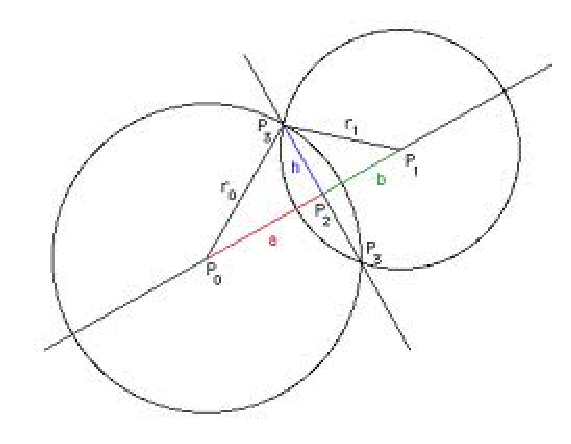
\includegraphics[scale=0.7]{intr.eps}
\caption{Circles intersection algorithm.\cite{cshint}}
\label{fig2}
\end{figure}

With two fixed points as the centres and distances to them as the radii we can draw two circles.
The circle should intersect at one or two points.
However, since there is interference in the measured RSSI values and thus the radii, it is also possible that the circles do not intersect.
The algorithm used to find intersections between two circles is a vector geometry based approach (Figure \ref{fig2})\cite{cshint}.

We observed that under measurement occurs more frequently than over measurement in RSSI values.
Therefore, we added 2 meters compensation to radii before calculating the intersections.

The playground is considered a two dimensional surface.
One Arduino node is at (0,0) and the other is at (10,0).
The target region is modelled as a rectangle.
Its upper left corner is at $(x, -H)$ and its lower right corner is at $(10-y, H)$, where $H$ is at least the ``width´´ of the playground.
The positive direction of axis in Java geometry library is lower right.
We are in the target region if any of the intersection points falls within the rectangle.

\section{Experimentation Setup}

\subsection{Implementation on Android Phone}

Using LG nexus 4 phones and Android development tools, we developed test applications that continuously scan for BLE devices using Android 4.3 BLE API. The GATT profile is a general specification for sending and receiving short pieces of data known as "attributes" over a BLE link. All current Low Energy application profiles are based on GATT. GATT is built on top of the Attribute Protocol (ATT). This is also referred to as GATT/ATT. ATT is optimised to run on BLE devices. Each attribute is uniquely identified by 128-bit format a Universally Unique Identifier (UUID). The attributes transported by ATT are formatted as characteristics and services.

\subsection{Arduino with BLE shield}

Bluetooth Low Energy Shield has been used to interface Arduino with Android device. It works with all Arduino boards, including Arduino Uno, Mega 2560, Leonardo, and Due. 

\subsection{Scenario}

\begin{figure}[h!]
\centering
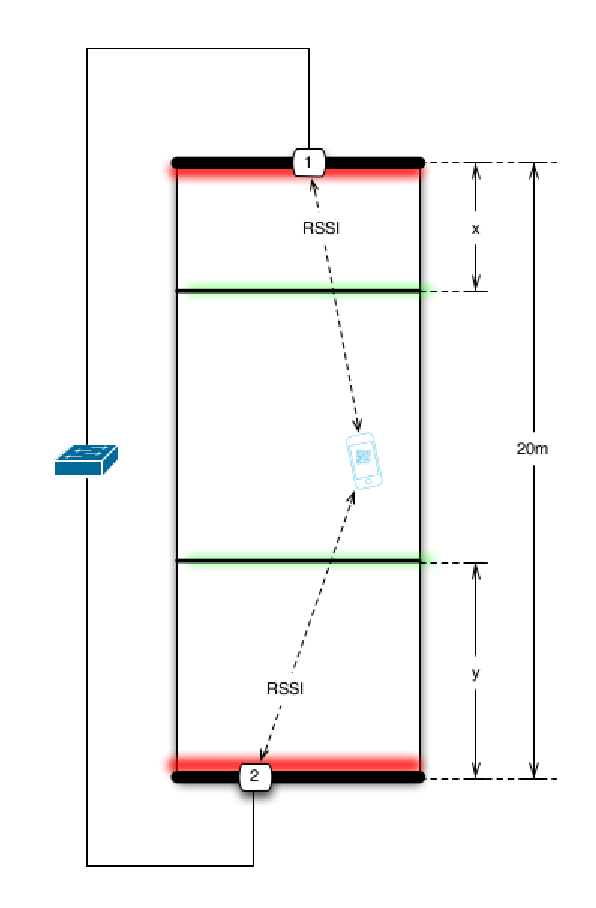
\includegraphics[scale=0.5]{position.eps}
\caption{Experimental Setup}
\label{fig1}
\end{figure}

The system (Figure \ref{fig1}) consists of two Arduino nodes located at two fixed positions and continuously scanning for Bluetooth LE (BLE) devices in the home area. These two stationary nodes calculate the distance between them and the other Bluetooth LE devices.
When the phone enters the region between green marks it signals the Arduino nodes to light up their LED.
When it leaves the region it signals the Arduino nodes to turn off their LED.


\subsection{Calibration}

First, we place one Arduino device at 1 meter distance from Android phone, scan 10 times and store RSSI samples.
We take the mean of these RSSI samples and calculate A.

\begin{equation}
 A = -meanRSSI_{at 1m}
\end{equation}

Then we move the phone to 2 meters away from the Arduino device and compute the value of n.
The same process is repeated for the other Arduino device to determine its A and n values.

\begin{equation}
 n = -(\frac{ meanRSSI_{at 2m}-A}{10 \log_{10}d})
\end{equation}


\subsection{Operation}

The communication between phone and the Arduino nodes are done through TCP/IP network.
Our Arduino boards are equipped with an Ethernet port.
We used a home router with Wi-Fi capability to connect Arduino node and the phone in the same IP network.

The Android application is based on the official Bluetooth LE sample and operates in a semi-automatic fashion.
Each time the user taps ``Scan´´ the application initiates a device scanning.
Android Bluetooth LE API provides also RSSI values for each discovered device.
Next, the user taps ``Report´´ and the application performs noise filtering, compute the intersections, and checks the target region predicate.

If it is determined that the phone is within the target region the application sends one HTTP request to each of the Arduino node with ``Z´´ as the requested resource.
Otherwise ``X´´ is the resource requested.
The Arduino nodes turn the LED on or off according to the resource requested in incoming HTTP requests.

Currently, all parameters such as IP address, Arduino node position, playground geometry, and target region are hard-coded in the Andriod application and Arduino software.

\section{Result}

In the demo, our design achieved reasonable precision until we are two meters from the boundary of the target region.

The playground is ten meters in length and the target region is bounded by the lines lying two meters away from each Arduino node.
The demo was conducted in an comparably open space than our development laboratory.
Multipath and other interference may be lower, which leads to better calibration and operation result than we anticipated.


\section{Analysis}

This work was based on Bluetooth positioning. After experimentation, we can conclude that it is not quite as easy as detecting the signal strength. Accurate and precise results depend on many factors, even what kind of phone we used in our experiment, the environment and how it might effect the signal strength, and also obstacles that may interfere with the signal, such as people, walls, tables. Additionally, phone orientation at a particular place experienced different RSSI values.

During address discovery system, the presence of many other devices (that are not part of the system) might 
increases probability of getting accurate and precise RSSI samples. However, as we noticed that the signal strengths significantly varied, we planned to do a lot of calibration. Calibration itself was not sufficient enough to determine the precise distance. Therefore, the RSSI value can estimate distance that might be basic near or far result. 

\section{Conclusion}

We find that this assignment is interesting and inspiring.
However, the Bluetooth LE API of both Android and Arduino are under documented.
The Bluetooth LE shield and built-in Ethernet module of our Arduino boards are sharing the SPI bus but with different parameters.
It took us quite some time to sort all of them out.
Since Android Bluetooth LE API only becomes available in the recent release, there was no official sample application from the manufacture of our Bluetooth LE shields for reference.

Both our experiment results and previous works suggests that using Bluetooth LE signal strength for precise positioning is likely unfeasible.

Our implementation is available at: \url{https://github.com/zwuh/heat_ble/}.

The authors would like to thank Vu Ba Tien Dung for his guidance throughout this project.




% trigger a \newpage just before the given reference
% number - used to balance the columns on the last page
% adjust value as needed - may need to be readjusted if
% the document is modified later
%\IEEEtriggeratref{8}
% The "triggered" command can be changed if desired:
%\IEEEtriggercmd{\enlargethispage{-5in}}

% references section
\nocite*{}
\bibliographystyle{../../sty/IEEEtran}
\bibliography{ble}


\end{document}

